% 来源：OEBPS/Text/Section0001_split_001.xhtml#sigil_toc_id_15

\BookChapter{6}
\section[第6章\q 哄来13万亿美元的营销谎言1：“把投资交给我们管理，我们能够战胜市场”]{第6章\\ 哄来13万亿美元的营销谎言1：“把投资交给我们管理，我们能够战胜市场”}

\begin{BookQuote}
非专业投资者的目标不应该是挑选牛股——不论是他还是他的帮手（投资顾问和基金经理都不能做到），而应该是同时拥有所有代表性企业的股票。总体而言，肯定会表现得很好，一个低成本的指数基金，就可以达到这个目标。

\hfill ——沃伦·巴菲特（《2013年致股东的信》）
\end{BookQuote}

\begin{BookQuote}
你看一看扣除费用和税收之后的净收益，就会知道在比较长的期限内，你几乎没有可能战胜指数基金。

\hfill ——戴维·斯文森（耶鲁大学的首席投资官，管理捐赠基金超过239亿美元）
\end{BookQuote}

\subsection{财经娱乐}

现在你打开电视上的财经频道，你看到的“新闻”很少，耸人听闻的事件很多。荧幕上都是大大的脑袋特写，他们在激烈地争论。那些推荐股票的主持人和专家，高声尖叫着当天的热门股，他们的声音从我们家客厅的音响里传出来，就像摔碎盘子、碟子一样尖锐混乱。记者就直接站在股票交易所里，进行现场报道。这套宣传体系是由广告商来付费的，目的就是要让你看了这些节目后形成一种感觉，我们就要错过机会了！只要我听了专家的热门股建议，肯定会赚钱。我听了专家的建议购买了这只基金，它肯定会成为下一个五星评级基金。（基金权威评级机构晨星公司对基金进行评级，最低是一星，最高是五星。）

追逐业绩排名是一门大生意。个人理财作家简·布莱恩特·奎因曾经把这种大肆宣传业绩排名的做法称为“金融业色情宣传”。它勾引我们去看那些印得非常精美的广告插页，只不过是把美女照片换成了五星级评级基金，或者换成了暗示你买了基金就能赚大钱、享受美好生活的照片，比如，无忧无虑地在沙滩上漫步，跟我们的孙子孙女一起坐在游艇的甲板上钓鱼。其实这些基金广告宣传的真正意图是，想要拿走我们口袋里的钱。各家基金公司争夺你财产的战争非常猛烈。

那么你把你的钱放到哪里呢？你能够信任谁呢？谁会保护你的资金安全，并为你的投资创造最好的投资收益呢？

这些问题，你马上就要考虑了。因为你现在已经承诺要把自己的收入拿出来一部分储蓄，去做投资了，你承诺自己要成为一个投资者了。那么大多数人把他们储蓄的钱投资到哪里去做长期投资了呢？一般是投到股票市场。

过去100年，股票市场确实是长期投资最好的地方。史蒂夫·福布斯参加了我在爱达荷州太阳谷举办的一场投资理财活动，那是在2014年。他说：“1935年在股票市场投资100万美元，到2014年，100万美元能够增值到24亿美元。你如果能一直持有，就能赚2400倍。”

但是，你开立了个人退休金账户或者参与了公司的401(k)退休金投资计划后，马上会有一个能说会道的营销员（或者销售流程）打电话给你，建议你把这些钱投资购买基金。表面来看，你买了一只主动管理型基金，实际上你真正购买的是什么？你其实买的是人，是基金经理。你付管理费给基金经理，希望他的选股能力胜过自己。这是一个非常自然的前提假设，因为我们这些业余投资者天天为工作和生活忙得不可开交，我们自己选股的那一套方法很低级，和朝着股票代码一览表乱扔飞镖差不多。

于是，我们把自己的钱委托给那些得到最高五星评级的主动管理型基金经理。顾名思义，主动管理就是主动积极地采取行动，努力追求战胜市场，其方法是让基金经理成为一个比别人更好的选股高手。有时我们称这是一个价值13万亿美元的谎言（因为投入主动管理型基金的资金规模高达13万亿美元）。你准备好直面这个13万亿美元的最大投资营销谎言了吗？

在一段较长的持续时间里，96\%的主动管理型基金未能战胜市场。如此高的失败比例，简直令人难以置信。

说得更清楚一点，我们说的“战胜市场”是总体而言的，我们说的市场一般是用一只股票指数作为代表的。你会问：什么是股票指数？有些人也许知道，但是我担心还有些人并不知道，要是不解释，这些人会听不明白，所以我先来解释一下股票指数。股票指数其实就是从所有上市公司中选择出有代表性的一篮子股票，或者说是一组股票，计算这些样本股的价格平均数。美国最常用也是最有名的股票指数是标准普尔500股票指数。其实就是标准普尔公司选择出来的500家顶尖上市公司，作为构成指数的成分股。主要的成分股有：苹果、埃克森美孚、亚马逊等。每天标准普尔公司会评估所有500只成分股的股价表现，把它们作为一个整体计算其最新价格，这就是我们看到的指数。你晚上听到新闻报道说股市上涨了或者下跌了，说的就是指数上涨了多少点，或者下跌了多少点。

你要追平股市就是要追平指数，那就要分别购买所有500只成分股，成分股变了，你还要跟着调整，卖出被剔除的成分股，买入新加入的成分股，这相当麻烦。有了指数基金，一切都非常简单了。你只要购买一只低成本指数基金，因为指数基金就是追踪或者复制指数，你的钱和成千上万的投资者的钱就会聚集到一起，其规模很大，可以用和指数同样的比例同时持有所有500只顶级上市公司的股票。只要购买一份指数基金，你就可以拥有整个“美国市场经济”的一小部分。用这种指数投资方式，其实你购买的是整个美国经济体系，你的信心来自100年的历史事实：过去100年，美国最强大的500家上市公司一直显示出了不可思议的活力。即使遇到经济衰退和经济大萧条，甚至是世界大战，它们也一直能够找到办法来增加价值，增长业务，提高收入。如果一家公司表现不好，不能进入前500名，标准普尔公司就会把它剔除出500只成分股的名单，用其他股价表现更好的上市公司代替。

这里我想讲的关键点是投资指数基金，你就不用再付钱给专业投资者帮你选股了。其实你已经选好股票了，因为标准普尔公司选择500只成分股时，就已经选择了表现最好的500家上市公司。顺便说一下，其实还有各种不同的指数。我们很多人都听说过道琼斯指数。我们很快会讨论分析其他指数。

\begin{figure}[htbp]
\centering
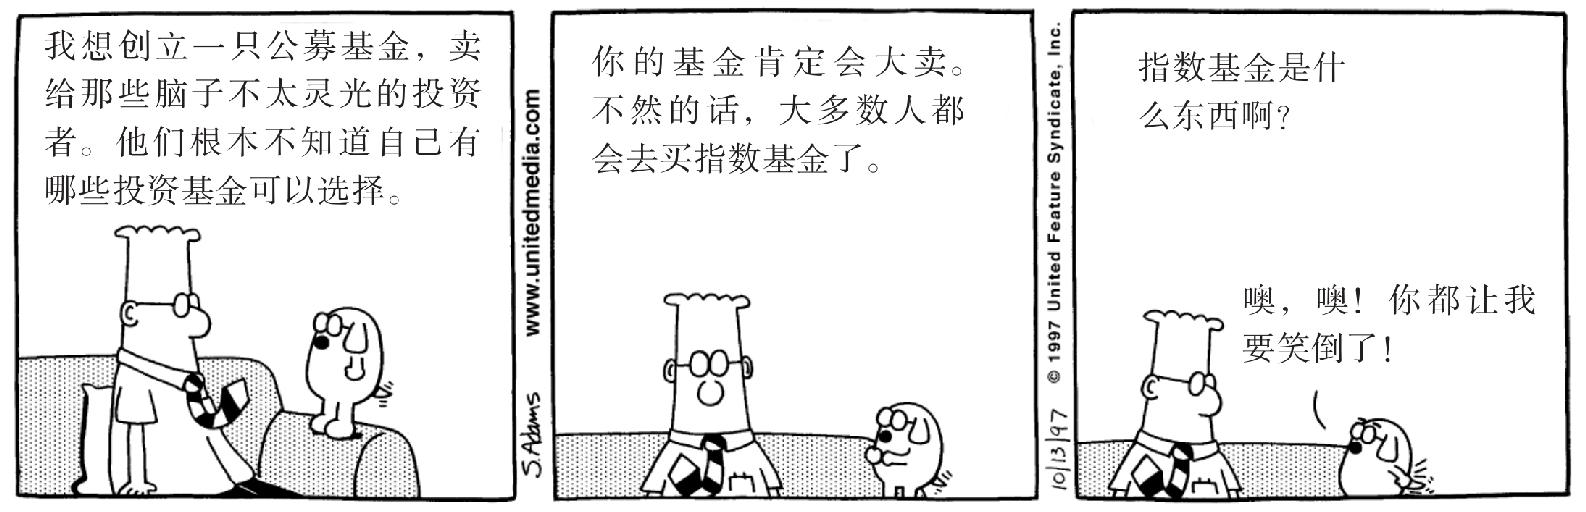
\includegraphics[width=0.98\linewidth,keepaspectratio]{image/6-1.jpg}
\caption{}\label{fig:6-1}
\end{figure}

\subsection{10000种选择}

目前美国有7707只各种各样的基金。你知道吗？基金比股票还要多，美国股市只有4900只股票。所有这些基金都在竞争，抢夺为你管理投资的机会，它们都说自己能够帮你战胜市场。但是统计数据就摆在那里，值得我在这里再重复一下：96\%的基金业绩未能追平市场或者战胜市场，在任何一段持续的时间里都是如此。这是不是令人震惊的大新闻？不，对于投资圈里的人来说，这根本不是新闻；对于机构来说，这也根本不是。瑞·达利欧特别强调：“你不要想去战胜市场！没有人能战胜市场！只有极少数人能获得金牌。”他碰巧正好是极少数投资比赛金牌的获得者之一，而且他非常诚实，才会向我们发出这样的严重警告。业余投资者根本别想战胜市场。

甚至是沃伦·巴菲特——尽管他以发现价值被低估的股票的神奇能力而闻名于世——也警告说，普通投资者根本不要想选股或者选股战胜市场。在他著名的《2014年致股东的信》里，巴菲特解释说，当他去世之后，他的作为信托留给妻子的钱，只能投资于指数基金，这样可以让成本最小化，让潜在的收益最大化。

巴菲特非常确定，即使是专业的选股者，长期来看也不能战胜市场。他的嘴怎么说，他的钱就会照做，他言行一致。2008年1月，巴菲特打了一个百万美元的大赌，对家是纽约的门徒投资合伙公司，最后的赢家可以把自己赢得的这100万美元，全部捐赠给自己指定的慈善组织。他们赌的是什么？门徒基金挑选了5只顶尖的对冲基金（中国人更多地称之为私募基金），赌它们未来十年的整体业绩能不能跑赢标准普尔500指数。目前十年赌局已经过去了6年，到2014年1月，标准普尔500指数6年上涨了43.8\%，5只对冲基金6年上涨了12.5\%。尽管十年赌局还未到期，但是指数基金领先的优势很大，就好像是世界上跑得最快的人博尔特跟一群小孩赛跑一样。（有些人可能不太了解对冲基金，其实本质上就是私募基金，非公开募集，客户只限于那些高净值人士，即财富非常多的人。对冲基金经理拥有完全的投资操作灵活性，既可以“做多”，市场上涨会赚大钱，也可以“做空”，市场下跌也会赚大钱。）

\subsection{事实就是事实，无可争辩}

金融行业研究专家罗伯特·阿洛特，研究大联盟的创始人，花了20年的时间研究业绩排名前200且管理资金规模超过1亿美元的主动管理型基金。结果令人震惊：1984—1998年，一共15个完整的年度，200个基金经理中只有8个人战胜了标准普尔500指数。（先锋500指数基金，是由先锋公司创始人约翰·博格创立的，是历史上第一只指数基金，它完全复制标准普尔500指数。）

也就是说，你想从这200只基金里面选出战胜市场的8只基金，概率为4\%。你要是玩过“21点”的扑克牌游戏，就知道游戏目标是让你的牌的合计点数尽可能接近21点，但是不能超过它，不然牌就爆了。丹·希思和奇普·希思兄弟两人在《快公司》杂志上发表了一篇文章，题目是《黏住客户：公募基金的谎言》。兄弟俩写道：“打个比方，你玩21点，已经翻开了两张牌，它们都是10，这样你总共是20点，那么你内心有个傻瓜在高喊：‘再要一张，大赢一把！’你有8\%左右的机会能赢！”

那么追逐业绩排名把我们伤得有多惨呢？从1993年12月31日到2013年12月31日，20年的期限，标准普尔500指数平均年化收益率是9.28\%，但是公募基金投资者的收益率只有2.54\%。这是业内领先的研究机构达尔巴的研究结果。天啊！基金投资人比市场平均业绩要低近80\%。

在现实生活中，这意味着财务自由跟财务绝境的巨大区别。换种方式，用数字说话，如果你觉得自己就是一个普通人，投资策略很简单，就是持有标准普尔500指数基金，那么你刚开始投资10000美元，过了20年，投资升值到55916美元，财富增长了5倍多。如果你因为听信了基金公司的营销广告，买了公募基金，觉得把钱交给基金经理管理可以战胜市场，那么你同样投资10000美元，20年后，它只能变成16386美元，财富增长不到2倍。

为什么差别会这么大？

原因是我们总想低买高卖，结果总是高买高卖。我们跟着自己的感觉走，或者跟着自己的情绪走，或者跟着股票经纪人、银行理财经理的建议走，从这只基金跳到另一只基金，跳来跳去。我们总想抓住一只业绩更好一点儿的基金。但是当股市下跌的时候，我们再也忍受不了账面损失所带来的情绪上的巨大痛苦，然后就把基金低价抛售了。但当市场上涨时，我们又会大量高位买入。正像一个著名的基金经理巴顿·毕格斯所说的那样：“牛市就像性爱，快要结束的时候感觉最爽。”

\begin{figure}[htbp]
\centering
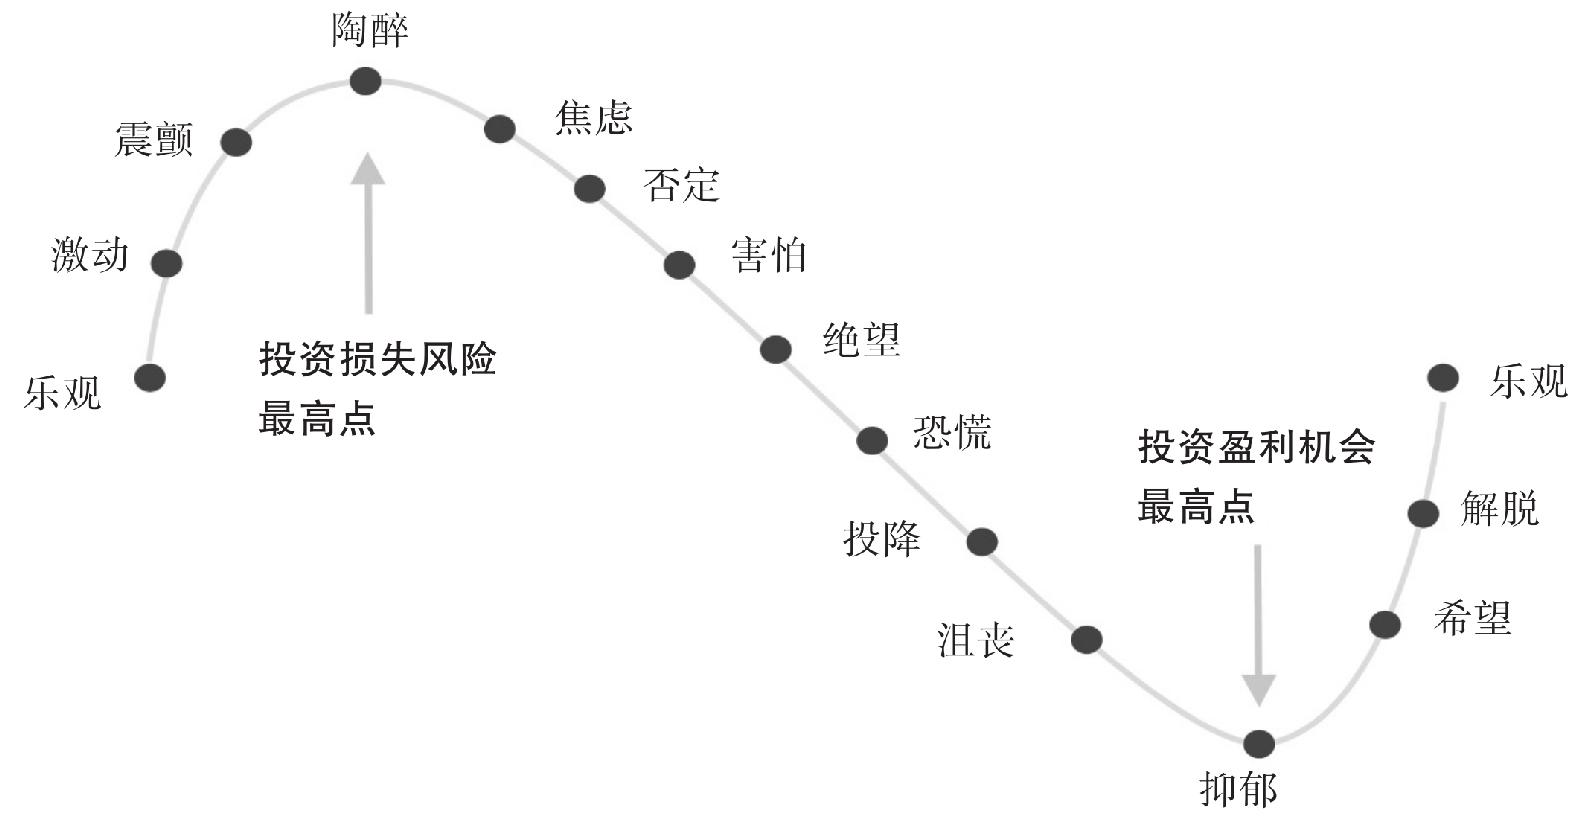
\includegraphics[width=0.90\linewidth,keepaspectratio]{image/6-2.jpg}
\caption{}\label{fig:6-2}
\end{figure}

\subsection{年纪越大，智慧越多}

现在已经82岁高龄的伯顿·麦基尔，经历过你所知道的每一种市场波动周期和市场风潮。1973年他在写《漫步华尔街》这本书时，根本没有想到它会成为历史上最经典的投资名著之一。这本书的核心理念是，在股票市场择时是一个输家的游戏。本书第四部分记录了我采访麦基尔的内容，听他分享一生的投资智慧。现在，你需要知道的是，麦基尔是第一个提出指数基金概念的人，即不要试图战胜市场，而要追平市场，或者说简单地“复制”市场。

现在，投资者都知道这种策略叫指数投资，也叫被动投资。这种投资风格与主动投资完全相反。主动投资是你付给一个基金经理管理费，让他主动积极地做出选择，买入某些股票或者卖出某些股票。这个基金经理不停地买进、卖出股票——“主动积极地”工作，希望能够战胜市场。

后来，约翰·博格创立了先锋公司，就把这家公司的未来发展方向押到了这个投资理念上，创造出了全球第一只指数基金。我去采访博格，问他先锋公司为什么会成为全球资产规模最大的指数基金管理人，他的回答铿锵有力：“最大化分散限度，最小化成本费用，最大化税收效率，降低换手率，降低换手成本，没有销售佣金。”他说得像“电梯游说”一样简短有力！

\subsection{捷径}

读到这里，你可能会想，肯定会有一些人能够战胜市场。要不然，怎么会有13万亿美元的资金购买主动管理型基金？基金经理确实会有一段时间顺风顺水，业绩跑赢市场。但是问题是他们不能把这种领先的优势长期保持下去。正如约翰·博格所说的，最后都是“营销”！人的本性就是想要比别人更快、更好、更聪明。所以卖一只热门基金一点儿也不难。业绩好，排名领先，自然有人抢着买。但是当这些热门基金的业绩变得不好，变成冷门基金时，马上就会有别的业绩好、排名高的热门基金出现，于是又出现一波疯狂的抢购。

我们前面说过只有4\%的基金经理能够战胜市场。但是，战胜市场的4\%的基金经理是完全不同的人。博格给我解释了这一点。他表述的方式非常好玩儿：“托尼，如果你能找到1024只大猩猩，把它们聚集到一家体育馆，教它们抛硬币，会有一只大猩猩连续10次正面朝上，成为冠军。大多数人会说这只大猩猩只不过是运气好而已。但是如果这种事发生在基金行业，我们就会称这家伙是天才。”那么同样还是这只大猩猩，接下来又连续10次抛硬币，其都是正面朝上的概率能有多大呢？

2013年诺贝尔经济学奖获得者尤金·法玛为三维基金顾问公司做了一项研究，其中有句话说得好：“现在还有什么人相信市场无效呢？很明显，只有朝鲜人、古巴和主动管理型基金经理。”\footnote{\label{fn:pdf-6-1}主动管理型基金经理依赖于自己的判断和经验来做投资决策，选择哪些股票和债券，买入、持有，还是卖出。他们相信用这种方法有可能战胜市场。}

那些在金融服务行业工作的人，读到这个部分，要么点头表示赞同，要么想利用这本厚厚的书敲开某公司的门，找份新工作！有些金融从业人员正搜集各种各样的武器进行反击。这毫无疑问是一个非常极端的观点。我们都相信，聘用世界上最聪明、最有天赋和才华的基金经理，能让我们更快地实现财务自由。毕竟，谁不想找条捷径快速登上顶峰呢？下面就是最疯狂的事：

每个人都有权发表个人意见，没有人有权否认自己看到的事实。

的确，有些基金经理会说：“牛市的时候，我们也许无法跑赢市场。但是，熊市的时候，我们可以主动采取措施来保护你的资产，让你的基金净值比市场跌得要少。”

如果是真的，嗯，这确实会让投资者感觉舒服很多。

投资的目标是在承担既定风险程度的前提下（理想情况是承担的风险水平最低）得到最高的净收益。让我们来看看，在股市下跌的时候基金经理是怎么做的。2008年金融危机，股市暴跌，先分析这段历史是最合适不过了。

2008—2009年年初，美国股市一年的跌幅创下了大萧条之后的历史之最（准确地说是从最高点到最低点，下跌了51\%）。对冲基金经理有足够的时间来做出防御行动。当市场下跌15\%，或者25\%，或者35\%的时候，他们都可以采取适当的措施。再一次，我们让事实说话。

不管基金经理是想击败标准普尔成长股指数（成分股有微软、高通、谷歌等），还是想击败标准普尔小盘股指数［成分股有Yelp（美国最大点评网站）等］，这些专业选股人再次跑输指数，根据2012年的研究报告《标准普尔指数与主动管理型基金业绩对比》，标准普尔500成长股指数跑赢了89.9\%的大盘成长型基金，而标准普尔500小盘股600成长指数跑赢了95.5\%的小盘成长型基金。

\subsection{独角兽}

现在我已经清楚地说过，几乎没有任何人可以长期战胜市场。但现在我要举出一个例外。确实有一小撮基金经理做到了似乎根本不可能的事——持续战胜市场，但是他们是独角兽，凤毛麟角，他们是魔术师，市场巫师，就像绿光资本的基金经理戴维·埃因霍恩。1996年，他推出了自己管理的基金，累计赢利2287\%（这不是印刷错误），而且没有一年出现亏损。但是不幸的是，即使你知道有这些超级明星基金经理，对于普通投资者来说也没有什么用，因为这些超级明星基金经理的基金大门已经关掉了，不再向新投资者开放申购。瑞·达利欧的桥水基金已经超过十年不再接受新的投资者加入了，即使原来接受新的投资者加入的时候，它也要求至少投资1亿美元，而且拥有50亿可投资资产。我的天啊，这门槛可真高！

保罗·都铎·琼斯一直保持不亏钱超过28年。最近，他告诉他的投资者，要退回20亿美元给他们。他的目的是缩小基金规模，因为一只对冲基金规模太大，进出市场就变得更加困难——难以快速又轻易地买进卖出。速度变慢意味着投资收益变低。

听到这里，你也许开始想本书是来鼓吹对冲基金闪闪发光的业绩的，所以我有必要做出解释。截至2012年，连续5个年度，大部分对冲基金经理都跑输了标准普尔500指数。根据财经新闻网站Zero Hedge的统计，2012年基金平均业绩为8\%，而标准普尔500指数涨幅为16\%。2013年对冲基金平均业绩为7.4\%，而标准普尔500指数上涨29.6\%，创下了1997年以来的最高年度涨幅。我可以肯定，那些富有的客户自己买的对冲基金连大盘也跑不赢，他们肯定不会感到满意。让他们更加心痛的是，这些对冲基金每年还要收取2\%的管理费，再加20\%的业绩提成，而且真正拿到手的投资收益，你还要按照最高级别的税率交纳所得税。我的心好痛。

\subsection{全球最大银行的女掌门人}

无论是在生活的哪个方面，我总是在寻找规则的例外，这正是创造卓越成就的地方。玛丽·卡拉汉·厄道斯正好符合这个要求。在金融行业这个男人主导的领域，这个女人却爬上了金融世界的金字塔的塔尖。华尔街这个地方，业绩说话的声音远远高过其他任何言辞。厄道斯的业绩高得出奇。她持续取得突破性的业绩，让自己成为J.P.摩根资产管理公司的首席执行官，现在她监管的投资组合资产规模超过2.5万亿美元。是的，单位不是亿是万亿。

写本书的时候，我采访了厄道斯，我们交流得非常好。她分享了一些非常深邃的智慧，我们会在第六部分一起倾听。但是当我抛出那些学术研究成果，说这些成果都表明没有基金经理能够长期战胜市场时，她马上就提出异议，J.P.摩根公司的很多基金经理，过去十年，在他们各自不同的资产类型上面，都战胜了市场。为什么？她提供的这些基金案例在市场下跌的时候，亏损幅度都低于市场跌幅。她说，正是这个差异为他们提供了领先市场的优势。厄道斯和很多行业专家一致同意，某些欠发达或者新兴市场为主动型基金经理提供了一些机会去获得“优势”。他们有机会在新兴市场获得很大的优势，例如肯尼亚、越南。在这些新兴市场里，信息并不像美国股市那样透明，信息传播速度也不是那样快。厄道斯说，在这些市场中，像摩根大通这样的公司有巨大的影响力和资源，可以利用公司在当地的关系及时洞察最新的情况，形成价值巨大的看法。

按照约翰·博格的说法，没有任何实证研究可以证明，主动管理型基金在所有资产类型里更加有效，包括大盘成长股、价值股、核心股、中盘成长股，等等。但是事实确实表明，在这些新兴市场的确存在投资机会，有时能够让主动管理型基金战胜市场。这些基金未来能够继续战胜市场吗？只有时间能够告诉我们答案。我们确实知道每一个主动型基金管理者，从瑞·达利欧到摩根大通，都要努力战胜市场，但在某个时点他们肯定会出现错误。因此发展形成一套投资体系，进行合适的资产配置至关重要。我们会在第四部分讨论这一点。你自己具体选择什么样的投资策略，有待你自己做评估。不要忘了，还要考虑费用和税收（我们会在下一章详细讨论）。

\subsection{全天候投资策略}

你阅读本书的时候可能遇到牛市，可能遇到熊市，也可能遇到横向盘整市。谁知道呢？关键是需要你的投资做好准备，迎接时间的考验，做一个全天候投资组合。我所访谈过的投资大师，在行情好的时候和行情不好的时候都做得很好，未来我们可以肯定的是市场会上涨也会下跌。生活要幸福并不能只是等着风暴过去，还要学会在雨中跳舞。在生活中你要消除害怕遇到风暴的恐惧感，好让自己能够专注于做好最重要的事情。

\subsection{何时？何地？如何？}

那么，全天候投资组合是什么样的？“托尼，我该把钱投到什么地方？”

第一，你没有必要浪费时间自己选择股票或者自己选择业绩最好的基金。购买一只低成本的指数基金，让它占到你所有资产的一定比例，这是最好的投资方式，因为我们不知道未来什么样的股票会表现最好。你想想，这样投资指数基金多酷啊，只要这样被动投资，持有市场上所有股票，你就可以击败96\%的人称“投资专家”的公募基金经理和同样多的私募基金经理（对冲基金）。这样做你就可以完全解脱了，再也不用费心费力地选择牛股，也不用选牛基金了。就像约翰·博格告诉我的那样，投资会让你感觉有点违反直觉。长期成功的秘诀就是：“什么也不要做，老老实实地待在那里。”不要去战胜市场，而要成为市场。这样你就会站在胜利者的那一边，跟着市场一起不断前进，不断成长，不断扩张。

到目前为止，我们很多次提到“市场”或者标准普尔500指数。但是请记住，标准普尔500指数只是股票市场众多指数之一，股票市场只是众多金融市场之一。比如，我们很多人都听说过道琼斯工业平均指数。其实除了股票指数之外，还有其他市场指数，例如商品指数、房地产指数、短期债券指数、长期债券指数、黄金指数。每种指数购买的比例，至关重要，我们会在第四部分做深入讨论。那么，你想不想让瑞·达利欧来告诉你什么才是他认为的理想的资产配置？在本书后面他分享了投资策略，1984—2013年，他每年的投资收益率只是略低于10\%，85\%的时间里他都是赚钱的。事实上，2008年股市下跌了37\%，他的投资组合模式只下跌了3.93\%。我真希望2008年股市暴跌的时候，我已经知道了他推荐的这种投资组合。

你也可以听一听戴维·斯文森是怎么说的。正是这个人管理着耶鲁大学的捐赠基金，从10亿美元增长到超过239亿美元，平均每年收益率为14\%。在本书后面，他也分享了他认为的理想的投资组合。所有这些大师的非常宝贵的投资建议都会收录在本书第六部分中。

你如果只关注这些专家推荐的投资组合模式，但并不完全了解资产配置，这就像是在不结实的地基上建造房子。如果你还没有深入地了解你的目标，只关注投资组合，那你完全是在浪费时间。也许最重要的是，如果我们不能保护你躲开那些想要把你的财富拿走一大部分的投资营销人员，你就会输个精光。这正是我们要在这里揭开9种投资营销谎言的原因。这也是简单7步投资法的第二步，让你能成为一个投资“内行”，知道事实真相。你只有知道事实真相，才会真正生活得自由自在。

\subsection{成为明星基金很值}

我们前面把该讲的都讲了，证据表明主动管理型基金几乎不可能战胜市场，但是毫无疑问，有些人还是会说：“托尼，你不用担心，我已经做了很多研究，我只投资五星评级的基金，低于五星评级的基金我一分钱也不投。”噢，真的吗？

根据晨星公司的研究，2000—2009年年底，投资公募基金的资金约有2万亿美元，大概有72\%的资金都流向四星或者五星评级的基金。有些人可能不太熟悉，晨星公司提供基金评级的全套服务，晨星基金评级最流行最常见，它根据基金过去的业绩表现制定了一套五星评级体系。股票经纪人和银行理财经理指导你哪个会是下一个热门基金，他们眼睛盯着的，嘴里说的都是几星评级。

戴维·斯文森告诉我：“晨星基金的星级评级实在太重要了，以至基金评级低于4星了，基金公司很快就会出手消灭掉。”2008—2012年，27\%的美国国内股票投资基金和23\%的国际股票投资基金都消失不见了，它们要么是合并了，要么是清盘了。这是很常见的做法，消除那些基金糟糕的历史业绩记录，整个基金家族就只剩下历史业绩辉煌的明星基金了。

基金公司的套路是设立多只新基金，看哪一只表现好就重点扶持，大力宣传营销。其他表现不佳的基金全部安乐死。约翰·博格这样解释道：“一家基金公司开始时会同时孵化5只小基金。它当然努力想让这5只基金都能胜出。这当然不可能。结果过了几年，其中4只基金都不能战胜市场，只有1只基金确实表现很好。它会抛弃那4只基金，然后开始大力营销那一只做得特别好的基金，其卖点就是非常好的历史业绩。”

想一想，我们在自己的投资生涯里会采取这种做法吗？如果你选了5只股票，有4只下跌，只有1只上涨，难道你会假装自己从来没有选过那4只亏损的股票吗？你还会告诉你的朋友，看你选到了一只多么牛的大牛股，以证明你的选股水平和巴菲特的一样，你是选股高手。这不是打肿脸充胖子吗？

除此之外，这些获得四星评级和五星评级的基金后来都成了死亡之星。《华尔街日报》上有一篇文章对此做了深入研究，标题是“投资者上了基金星级评级的大当”。这份研究报告追溯到1999年，研究了那些购买了五星评级基金的投资者之后十年的业绩表现。研究的发现是什么呢？“在这十年里，初期获得五星评级的基金有248只，但是十年之后还保有五星评级的基金只剩下4只。”

有多少次你选了一颗冉冉升起的新星，却看到它在燃烧后突然坠落、化为灰烬，这些冉冉升起的新星98\%都会熄灭，坠入黑暗，只有2\%的新星会继续熊熊燃烧，我们都希望找到那个金手指，能够点股成金。但是历史表明那些金手指最后会变成铁手指，最终化为尘土。这正是拉斯维加斯永远会赢的原因。

投资内行都知道，追逐业绩排名很高的基金就像追逐风险一样，最后会落得一场空。但是，人类的本性决定了人们会追逐业绩排名很高的基金，这几乎是无法抵抗的诱惑，但是羊群心理最终导致数百万家庭的财富毁灭。我知道如果你正在读本书，你再也不愿成为这些明星基金的牺牲品，你正在努力成为投资专业人士。还有没有其他投资内行所用的很厉害的投资策略呢？让我们来找找。

\subsection{盈利有保障}

过去的100年里有70\%的时间，市场处于上升状态。但是还有30\%的时间，股市是下跌的。所以尽管对于你的一部分资金来说，指数投资是一个很好的解决之道，但是对于你的所有资金来说它并非最佳的策略，你不能把所有的资金都投到指数基金上。市场起伏不定，所以当市场再次出现暴跌时，你想保护你的投资组合的一部分绝对安全是很理智、很正常的。哎，从2000年到现在，股市已经两次腰斩了。

我们会给你介绍一个令人激动的策略：当股市上涨，指数上涨时，你能赚钱；当股市下跌的时候，它马上可以保证你的本金安全。这代表什么？你不用牺牲所有的投资收益。

大部分人根本不相信有这样的投资工具。为什么你从来没听说过？因为这些投资工具一般都是给那些高净值客户保留的，我会告诉你，告诉普通投资者能够找到这些投资工具的少数地方之一。想象一下你的朋友们疑惑地看着你的感觉，他们搞不明白为什么投资市场上涨时，你会赚钱，投资市场下跌时你也不会亏钱。只用一种投资策略就能完全改变你对投资的看法，这就像在你爬山时有条安全绳，而别人只能历经惊险和刺激，一路攀爬，只能向上天祈祷自己不会出事。想象一下那种确定的感觉，那种内心的宁静吧，因为你知道你没有处在风险之中。这会如何改变你的人生？当你每个月打开你的对账单时，你会有什么样的感觉？你是咬牙切齿，还是感到冷静和镇定？

这只是皮毛而已，后面我们要讲述的投资智慧和工具会让你觉得深不见底。所以你要一直保持热情，但现在我们可以先记住我们前面所讲的东西。

\begin{itemize}
\item 到目前为止，股票是做长期投资最好的地方。
\item 股票价格波动很大，后面你会学到如何抹平高峰和低谷，稳定地骑在马上。大师们的方法是投资多种不同的指数，让投资分散化、多元化。
\item 啊！很少有人会战胜市场。相反，我们要和市场站在一起。你只要做出投资计划，我们会教你一步一步地去做，你就不用再浪费时间去选股了，因为指数已经帮你做好选股了。这会帮你节省大量的时间和精力。
\item 开始像一个投资内行一样思考，再也不要容忍自己在投资生涯里出现那种羊群心理了。
\end{itemize}

\subsection{关于费用的费用}

通过引入指数投资的力量和被动地持有整个市场，你就会战胜第二个投资营销谎言。我问过很多人，几乎没有一个人准确地知道自己付的费用是多少。我承认，我自己也曾经根本不知道自己付的费用是多少。那些金融机构就是专门制造费用的工厂，它们的手法非常高明。它们要么把费用隐藏起来让你根本看不到，要么把费用包装得让你感觉数额很小，完全可以忽略不计。“没有什么大不了的。”这句话说得再确切不过了，一点儿小钱，你感觉无所谓。当你攀登财务自由的山峰时，你需要每一点儿资金，它能够让你多前进一点儿，更接近成功一点儿。要是进两步又退一步，因为那些过多的费用会吸干你一大部分投资收益，这可让你负担不起。真正的问题是，你赚的钱到底是进到了别人的退休金账户，还是进入了自己的退休金账户。翻到下一页，我们一起来找寻答案。
